
\section{The cuprate phase diagram}

The phase diagrams for the \highTc materials show a remarkable consistancy across the cuprates\footnote{This is in constrast with the recently discovered pnictide materials which show significant variations in scalings and even composition}. However this universality amongst the cuprates comes with an abundance of features which provide for some complex physical interactions and fragile intermediate `crossover' phases. The tuning parameter for the cuprate phase diagram is either electron or hole doping typically performed by elemental substitution at the crystal growth stage or by oxygen incorporation through annealing. as shown in figure~\ref{Fig:Intro:ElecHolePhaseDiagram}, the two types of doping are not symmetric with hole doping generally resulting in more robust superconductivity. For this reason the literature has largely concentrated on the hole doped preogression and as a result it is far better characterised. The doping is usually expressed as a $p$ value which represents the amount of additional holes (electrons) per Cu atom.
\begin{figure}[htbp]
    \begin{center}
        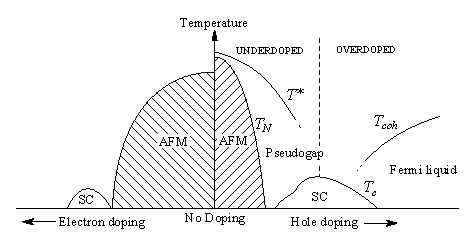
\includegraphics[scale=0.9]{Chapter-Introduction/Figures/ElecHolePhaseDiagram/ElecHolePhaseDiagram}
        \caption{A schematic phase diagram showing electron doped to the left and hole doped to the right. AFM is the antiferromagnetic Mott insulating phase, SC is the superconducting phase. $T^*$, $T_N$, $T_c$ and $T_{\textrm{coh}}$ are the temeprature scales for the pseudogap, AFM state, superconductivity and coherent Fermi liquid phases respectively}
        \label{Fig:Intro:ElecHolePhaseDiagram}
    \end{center}
\end{figure}

\subsection{Mott insulating parent compound}

Starting at the middle of figure~\ref{Fig:Intro:ElecHolePhaseDiagram}, the parent compound materials at zero doping are though to be Mott insulators i.e. the top most filled state on each lattice site contains one electron. In the conventional band picture this should be metallic since the bands are only partially filled, however when we consider a local picture of electrons, any movement of an electron to the neighbouring lattice site will cause an energetically costly double occupancy on one site and zero occupancy on another. This causes the electronic \ac{DOS} to become gapped around the Fermi surface and hence supressed conduction. This is known as the Mott insulating state.

We find that the kinetic energy term is reduced when the ordering of the sites is antiferromagnetic since for any hopping to occur at all, the spins must be antialigned to avoid double occupancy of like spins. This region dominates the low doping portion of the pahse diagram and remains antiferromagnetic until either the temperature is high enough to allow transitions from the Fermi energy to the states at the edge of the gap or the doping has introduced enough double occupancy electrons on lattice sites, which can move without the double occupancy energy cost, to overcome the insulating behaviour.

\subsection{Superconducting dome}

With increased doping, the antiferromagnetic state gives way to the superconducting dome at around $p=0.05$ which itself gives way to a Fermi liquid metallic state at a doping of around $p=0.3$. The maximum \Tc occurs at around $p=0.19$. Transitions from both the antiferromagnetic and the superconducting state are clearly second order thermodynamic with jumps in the heat capacity for example, however there are other regions in the phase diagram which are less well defined such as the pseudogap and the Fermi liquid crossover whose temeprature scale can depend on the particular probe used and do not feature a clear order parameter.

\subsection{Coherent phase}

To the heavily overdoped side of the phase diagram, beyond the superocnducting dome lies the coherent region where the system bears the hallmarks of a conventional metal. The implication is that correlations between electrons are sufficently weak such that the mass enhanced quasiparticles of Landau's Fermi liquid theory are well defined, leading to conventional metal behaviour. The clearest indication of this is a dominant $T^2$ term in the resistivity. Above this region we observe an anomalous additional contribution which has been modelled both with $T^2$ plus an additional linear term or by a $T^n$ term where $1 <= n <= 2$. This additional term has been observed before and is often associated with proximity to a \ac{QCP} for example in heavy Fermion materials.

\subsection{The pseudogap}

Above the \ac{AFM} region and the superconudcting state is one of the most contraversial regions of the phase diagram is the so called pseudogap phase. This is a region which was first demonstrated in 1989, just a few years after the discovery of the cuprate materials, by \ac{NMR} measurements performed at Bell labs~\cite{Warren1989}. A noticeable fall in the susceptibility occured at a temperature significantly above \Tc which led to conclusion of possible spin pairing before the onset of bulk superconductivity\footnote{Unpaired electrons contribute to the magnetic susceptibility response, Cooper paired electrons in the singlet state have zero net spin hence the explanation as to the reduction in susceptibility}. The question arose as to what the exact relation of the pseudogap is to the superconducting state --- is it a precursor state, from which superconductivity arises or is it a competing phase? --- and from a materials development point of view, to obtain higher \Tc should we be finding ways to suppress the crossover to the pseudogap state or encourage it?
\begin{figure}[htbp]
    \begin{center}
        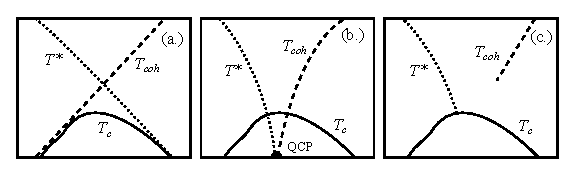
\includegraphics[scale=0.9]{Chapter-Introduction/Figures/PGScenarios/PGScenarios}
        \caption{Thre scenarios proposed for the $T^*$ temperature scale behaviour. (a.) the pseudogap as the `precursor' state, (b.) as the `competing' state, (c.) and the `transition' scenario.}
        \label{Fig:Intro:PGScenario}
    \end{center}
\end{figure}
By finding where exactly the $T^*$ energy scale meets the superconducting dome, strong evidence can be found that supports one or the other scenario. However the problem lies in the type of probe used. Select spectroscopic measurements including \ac{STM}, \ac{ARPES} and Raman on materials of camparable $T_C$ have found that the $T^*$ overreaches the superconducting dome entireley~\cite{Hufner2008}, meeting with the overdoped edge at $T=\unit{0}{\kelvin}$. This supports the precursor state theory illustrated in figure~\ref{Fig:Intro:PGScenario}(a.) where $T^*$ and $T_{\textrm{coh}}$ cross to define a region which is below both temeprature scales where the carrier are both paired and coherent quasiparticles leading to the superconducting condensate.

A second scenario is supported by measurements using bulk probes such as heat capcity, magnetic susceptibility and resistivity data have shown the $T^*$ energy scale drops into the top of the superconducting dome~\cite{Tallon2001}. This supports the scenario where the pseudogap is in competition with superconductivity for states at the Fermi surface. Once the pseudogap phase is suppressed, scattering from quantum fluctuations at zero temeprature leads to the formation of the superconducting phase at a \ac{QCP} similar to that found in heavy fermion materials. This scenario is supported by the observation of linear scaling of the resistivtity with temperature in the region above the superconducting domewhich is a hallmark of proximity of a \ac{QCP}.
% Kondo is a competitive scenario which justified based on
% non-monotonicity of coherence as you move from the antinodes on the FS \cite{Kondo2009}

A third scenario is one where the pseudogap simply becomes the superconducting gap as it meets the top of the superconducting dome. However this scenario leaves hanging questions as to the roles of the pseudogap, $T_{\textrm{coh}}$ and other phenomena in the phase diagram which would need to be addressed theoretically. Moreover this picture is rendered less compelling by the observation in LSCO of rapidly increasing, low temperature, normal state resistivity inside of the underdoped superconducting dome which implies the non-superconducting energy gap persists into this region.


\subsection{Previous work by the Bristol group}

Clearly lots of interesting physics is occurring in and around the superconducting dome and a solid understanding of this region is key to understnading the problem of high-$T_c$. Prof. N. Hussey has been involved in many efforts to shed light n the situation, of which, two key ones are highlighted here.

\subsubsection{Links between anisotropic scattering and \Tc}

Simply measuring resistance along different axes gives an averaged scattering rate and so to build a map of the angle dependent scattering rates, a different technique must be used. In \ac{ADMR} a strong persistant magnetic field is applied before resistance measurements are taken. The field serves two purposes; firstly, to suppress superconductivity so the normal state can be probed, secondly to confine the electrons to orbits perpendicular to the field. By detailed analysis of the change in resistance as the field is applied at various angles, a picture of the angle dependent scattering rate can be determined.

After performing measurements on samples of Tl$_{2201}$ with dopings ranging from strongly overdoped to slightly underdoped~\cite{Abdel-Jawad2006}, a trend emerged which is illustrated in figure~\ref{Fig:Intro:AnisotropyPhase}. 
\begin{figure}[htbp]
    \begin{center}
        \includegraphics[scale=0.9]{Chapter-Introduction/Figures/AnisotropyPhase/AnisotropyPhase}
        \caption{Schematic of how the scattering rate, $\Gamma$, the Fermi surface, $FS$, and the superconducting gap, $\Delta_g$ evolve with doping across the superconducting dome. Based on figure 1 in ref~\cite{Taillefer2006}. The dotted line in the scattering is the isotropic part.}
        \label{Fig:Intro:AnisotropyPhase}
    \end{center}
\end{figure}
Here the scattering rate within the $ab$-plane, $\Gamma$, was found to be composed of two terms; an isotropic term which remained constant with doping (dotted circle) and an anisotropic component which scaled with the superconducting gap, $\Delta_g$. Moreover it was found that the superconducting gap and the anisotropic scattering rate both shared the same shape, being `d-wave'. This further ties to \ac{ARPES} measurement which show that the on the underdoped side of the superconducting dome there is a Fermi surface reconstruction where at the antinodal points of $\Gamma$ (and $\Delta_G$) the spectral weight dissappears~\cite{Norman2010}. It changes from a single large hole band of volume $1+p$ to series of small regions of electron and hole Fermi surface of total volume $p$.

\subsubsection{T-Linear behaviour in the superconducting dome}

Previous high-field transport measurements on Sr doped LSCO~\cite{Cooper2009} gave key insights into the nature of the T-linear term as it entered the superconducting term on the overdoped side. In particular it showed that the T-linear term did not funnel down to a point (figure~\ref{Fig:Intro:CooperTLinear}) as is typical of \ac{QCP} behaviour but instead spread out into the superconudcting region. Intrigued as to this unexpected behaviour, we looked to repeat the measurements on \ac{BSCO} which can be doped far more widely without divergence in the resistivity so that we could then see how the T-linear term progressed on the underdoped side, where $T^*$ is undisputed.
\begin{figure}[htbp]
    \begin{center}
        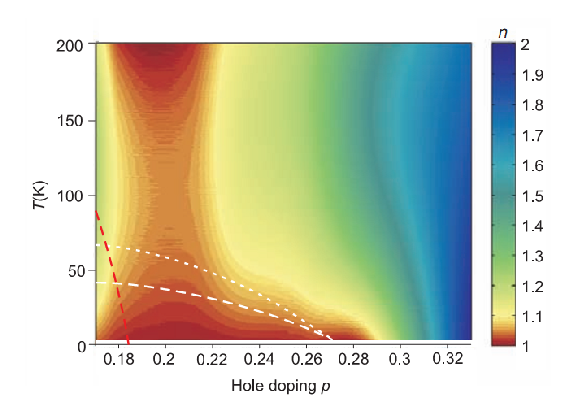
\includegraphics[scale=0.8]{Chapter-Introduction/Figures/CooperTLinear/CooperTLinear}
        \caption{Plot of the $T^n$ term in the fitted field suppressed normal state of Sr doped LSCO showing the $T$-linear term extending throughout the superconducting dome and not to a single \ac{QCP}. Taken from Cooper \etal~\cite{Cooper2009}}
        \label{Fig:Intro:CooperTLinear}
    \end{center}
\end{figure}
Performing meaurements which would shed light onto which of the scenarios shown in fig~\ref{Fig:Intro:PGScenarios} is most likely to be correct formed the original motivation for the the investigation of \ac{BSCO} through transport measurements. A second reason for the study of \ac{BSCO} is that it's van-Hove singularity occurs far from the doping levels that we are interested in unlike LSCO. Should similar behaviour be found then we can confidently state that the unsuaul \ac{QCP} behaviour is not due to proximity to the changeover in hole-like to electron-like Fermi surface and is likely universal to all cuprates. 

\ac{BSCO} also demonstrates trnaspotr behaviours which are consitent with other \highTc cuprate materials. For example, from \ac{MR} measurements it demonstrates a similar maximum in the underdoped $d\rho_{ab}/dT$ curve as underdoped YBCO~\cite{Ando1999}. On the overdoped side, \ac{BSCO} demonstrates a monotonic upward trend in $d\rho_{ab}/dT$ with increasing temperature similar to what has been observed in Tl$_{2201}$ and \ac{LSCO}~\cite{Ando1999}.

During the course of the ivestigations however, it became apparent that even with field strengths of up to \unit{60}{\tesla} in pulsed fields, the upper critical field, $H_{\textrm{c2}}$ of many of the sample at key temperatures could not be reached. However, field strengths were generally strong enough to recover $B$-Linear behaviour in the Hall component.

Previous Hall measurements have been performed on \ac{BSCO} by Ando \etal \TODO{todo}

% Motivation

% Lograithmic divergence of scattering rate observed in cuprates which
% begins at critical doping and increases as become more underdoped.
% However common factor of cuprates (Y123, Tl2201, LSCO) is a change of
% Fermi surface (in LSCO at least) from hole to electron leading to a
% van Hove singularity(?) which occurs similar to hwere would expect the
% insulating crossover. This does not occur in BSCO however until
% around p=0.2\cite{Hashimoto2008}. If the \alpha^2 term takes off
% earlier for BSCO\cite{Hussey2011a} is good
% evidence that is due to the proximity to van Hove rather  than Moot
% insulator transition.\cite{Ono2000}


% \section{Mott physics}

% The Hubbard model takes the relatively simple and solvable tight-binding model and introduces an Anderson term which raises the energy for double occupancy by an amount $U$, known as the `Hubbard U'. This simple change deeply enriches the physics with one of the outcomes being the existance of the Mott insulating state which occurs when each lattice site is half filled with a single electron. The energy cost for an electron to hop to an adjacent site is so high that it locks the electrons in place, preventing effective conduction. Introducing holes (or electrons) allows once again hopping to take place and the eigenstates are no longer entireley localised.
